

\setchapterpreamble[u]{%
\dictum[\LaTeX, 1. Gebot]{Thou shallst concentrate on the content}}
\chapter{\LaTeX~f�r TW-Dokumentation}


\newpage
\section{Allgemeines}
\subsection{\LaTeX}

Aus der \LaTeX-Doku:
\begin{quote}
LaTeX is a document preparation system for high-quality typesetting. It is
most often used for medium-to-large technical or scientific documents but it
can be used for almost any form of publishing.

LaTeX is not a word processor! Instead, LaTeX encourages authors not to worry
too much about the appearance of their documents but to concentrate on getting
the right content.
\end{quote}

Online Befehlsreferenz: http://www.weinelt.de/latex/index.html

\subsection{Einbindung der Vorlage}

\begin{enumerate}
\item svn: template.tex aus dem TeX-Verzeichnis ins eigene Handbuchverzeichnis
kopieren (e.g. FAS)
\item alte Zentraldatei (FASo.tex) umbenennen in FASo\_old.tex
\item Kopie von template.tex umbenennen in FASo.tex
\item Kapitel-includes aus FASo\_old.tex in FASo.tex kopieren
\end{enumerate}

\section{Bilder}
\subsection{Format}

\begin{itemize}
\item Screenshots im PNG-Format speichern
\item Benamsung: dokumentname\_kapitelname\_bildname.png\\
(e.g. CIS\_benotungstool\_notenschluessel.png)
\item Im Bildbearbeitungsprogramm Ausgabebreite auf 140mm stellen ->
errechnete H�he f�r picture - Umgebung wichtig
\end{itemize}

\newpage
\subsection{Einbindung}

\begin{figure}[htbp]
    \begin{center}
        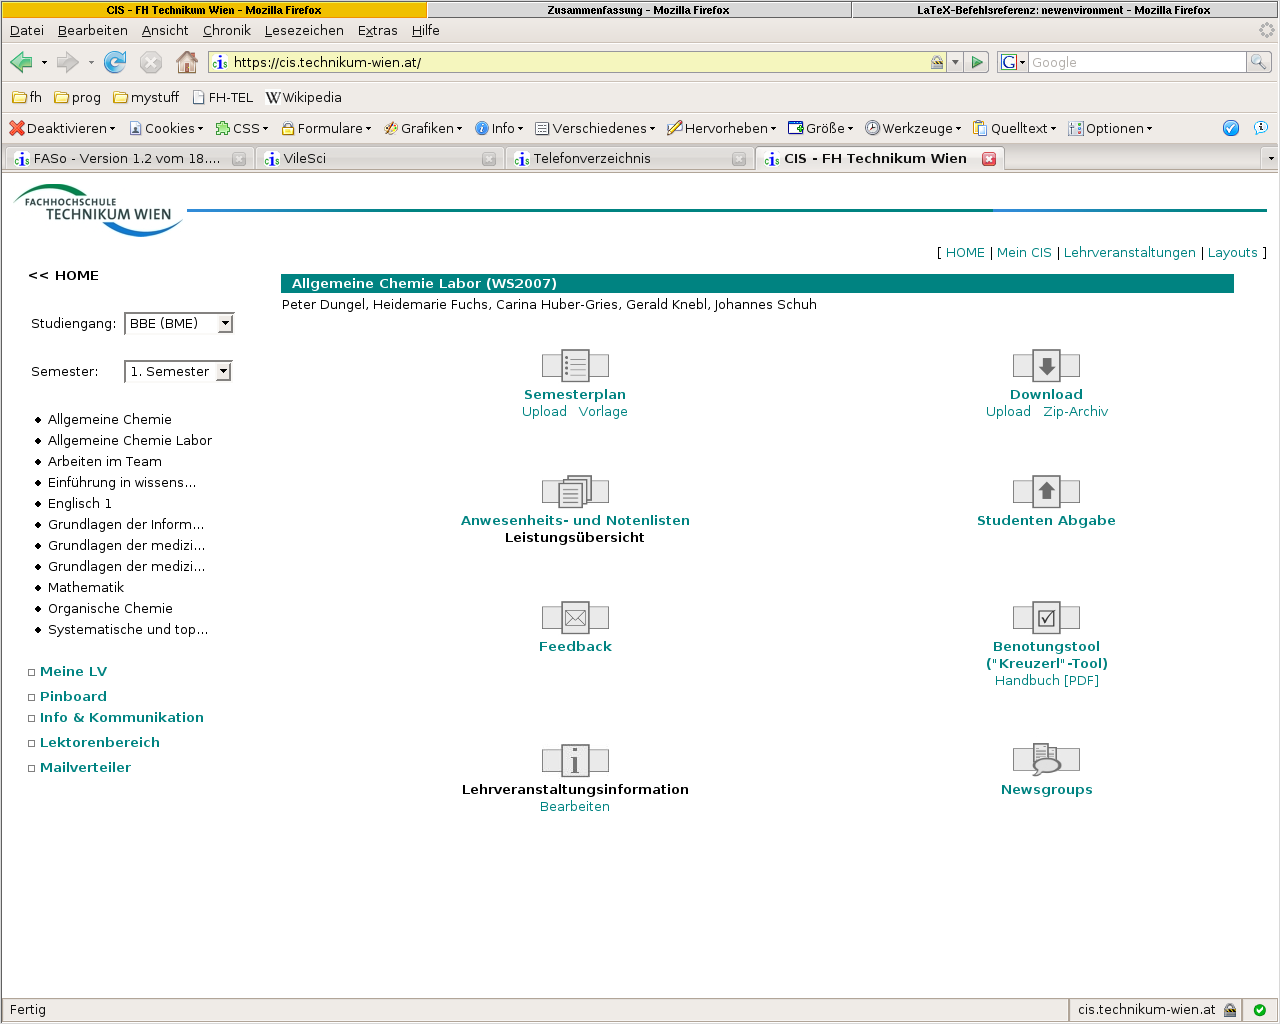
\includegraphics[width=0.9\textwidth]{dummy}
        \caption{Einfache Einbindung eines Bildes ohne Marker}
        \label{foo}
    \end{center}
\end{figure}

\begin{lstlisting}[caption=Code zu Abb. \ref{foo}]
\begin{figure}[htbp]
    \begin{center}
        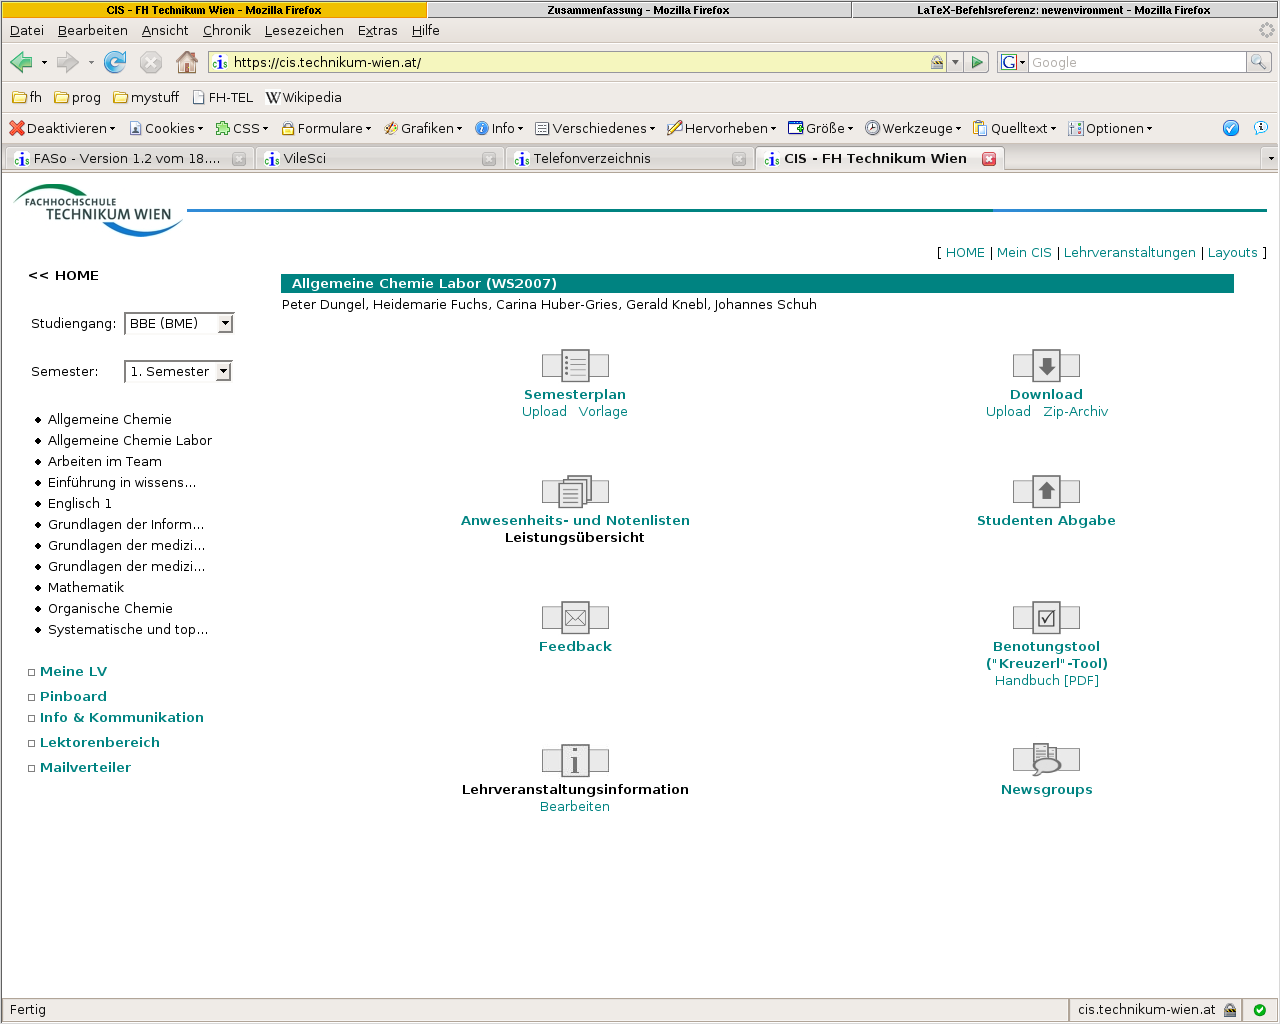
\includegraphics[width=0.9\textwidth]{dummy}
        \caption{Einfache Einbindung eines Bildes ohne Marker}
        \label{foo}
    \end{center}
\end{figure}
\end{lstlisting}


\newpage

\begin{figure}[htbp]
    \begin{center}
        \begin{picture}(140,112)
            \put(0,0){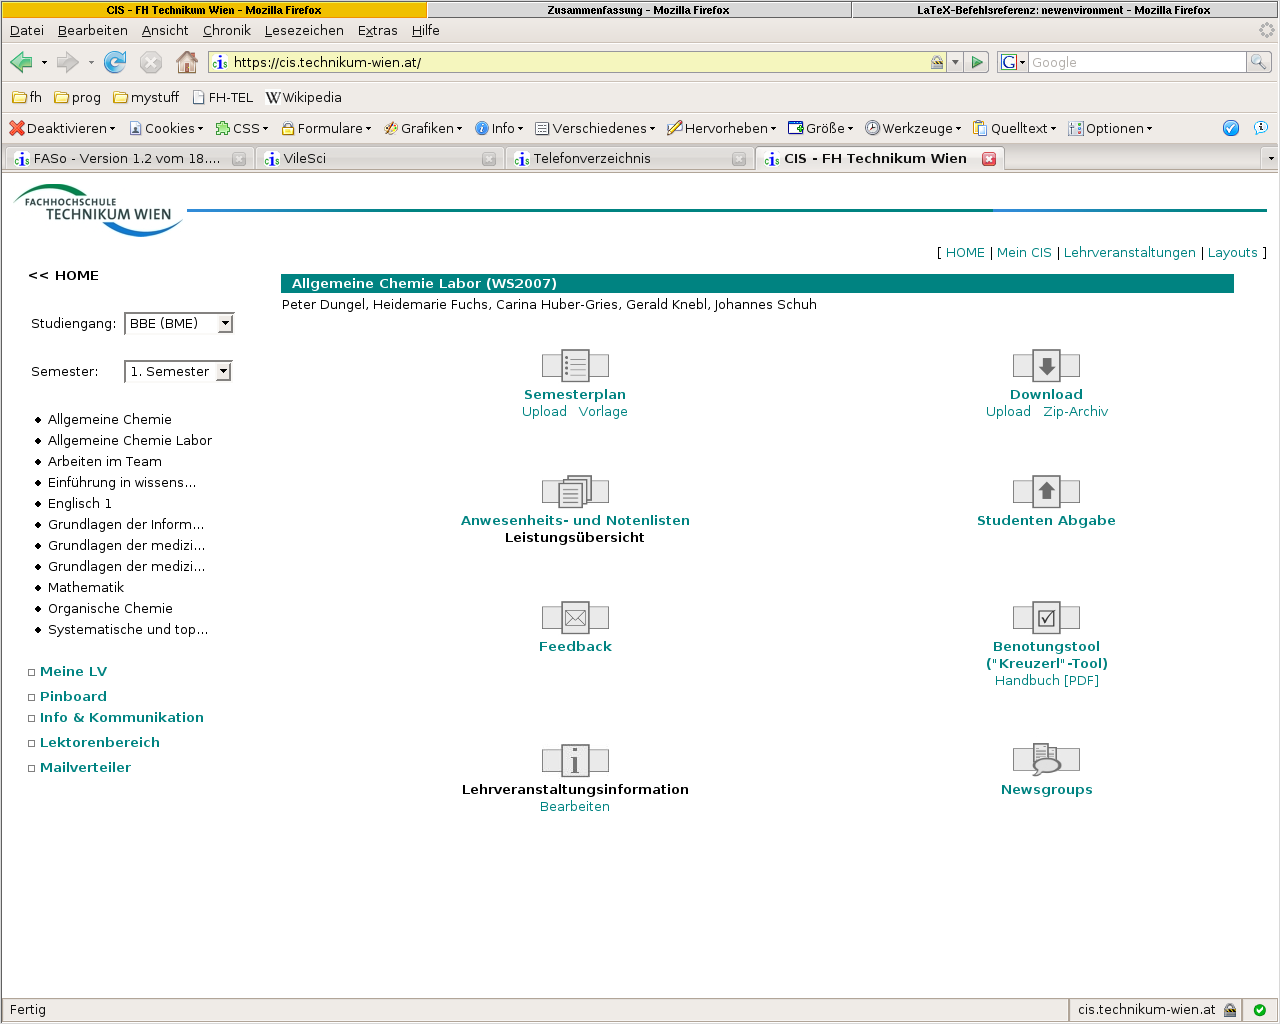
\includegraphics[width=140mm]{dummy}}
            \markier{1}{50}{36}{1}{1}
            \markier{2}{105}{36}{1}{-1}

        \end{picture}
        \caption{Einbindung eines Bildes mit 2 Markern}
        \label{bar}
    \end{center}
\end{figure}

\begin{lstlisting}[caption=Code zu Abb. \ref{bar}]
\begin{figure}[htbp]
    \begin{center}
        \begin{picture}(140,112)
            \put(0,0){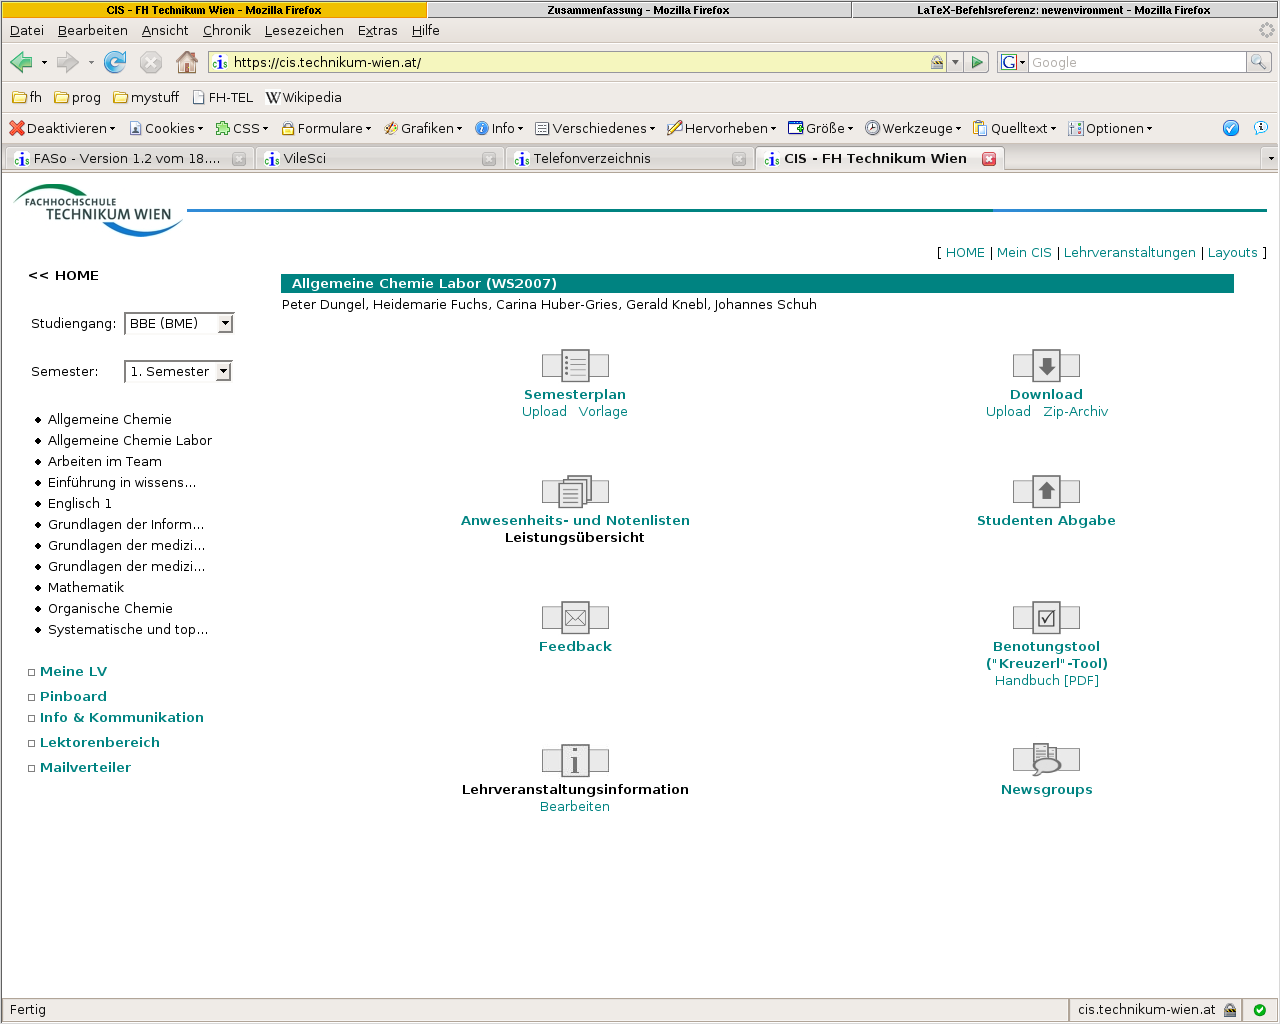
\includegraphics[width=140mm]{dummy}}
            \markier{1}{50}{36}{1}{1}
            \markier{2}{105}{36}{1}{-1}
        \end{picture}
        \caption{Einbindung eines Bildes mit 2 Markern}
        \label{bar}
    \end{center}
\end{figure}
\end{lstlisting}

Details zur markier-Umgebung:
\begin{lstlisting}
\markier{nummer}{x}{y}{vector_x}{vector_y}
\end{lstlisting}

\textbf{nummer}: dargestellte Zahl, \textbf{x, y}: Kreiszentrum von links
unten in mm, \textbf{vector\_x, vector\_y}: Steigung des Pfeiles: Zahlen von -4 bis +4

\achtung{Die H�he der picture-Umgebung muss dem Screenshot angepasst
werden!\\ Angabe in mm; hier: (140,\textbf{112})}

\subsection{Referenzierung}


\ldots\\
Feedback an den LV-Leiter k�nnen Sie �ber den Link \textit{Feedback} (s. Abb.
\ref{bar} Pkt. 1 auf S. \pageref{bar}) senden. \\
\ldots\\

\begin{lstlisting}[]
(s. Abb. \ref{bar} Pkt. 1 auf S. \pageref{bar})
\end{lstlisting}


\section{Boxen}

\achtung{Achtung!}

\idee{Idee, Tipp}

\halt{\textbf{HALT!}}

\info
{
    \begin{tabular}[t]{p{40mm}|cp{70mm}}
        \cline{1-3}
        9. Oktober 2007&-& Infomail der freigegebenen Noten beinhaltet nun auch die
        Note\\
        \cline{1-3}
    \end{tabular}
}

\begin{lstlisting}[]


\achtung{Achtung!}

\idee{Idee, Tipp}

\halt{\textbf{HALT!}}

\info
{
    \begin{tabular}[t]{p{40mm}|cp{70mm}}
        \cline{1-3}
        9. Oktober 2007&-& Infomail der freigegebenen Noten 
        beinhaltet nun auch die Note\\
        \cline{1-3}
    \end{tabular}
}

\end{lstlisting}

